\documentclass[a4paper]{exercisesheet}

%\usepackage{mathpazo}
%\usepackage{mathptmx}
%\usepackage{newtxmath}
\usepackage[T1]{fontenc}
\usepackage[utf8]{luainputenc}
\usepackage[charter]{mathdesign}
\let\sfdefault=\rmdefault
\def\ttdefault{txtt}

\usepackage[dvipsnames]{xcolor}
%\colorlet{maincolor}{blue!50!black}
\colorlet{maincolor}{black}

\usepackage{listings}
%\lstset{
%  frame=lines,
%  backgroundcolor=\color{maincolor!15},
%  rulecolor=\color{maincolor},
%  language=Python
%  keywordstyle=\bfseries\color{maincolor},
%  numbers=left,
%  numberstyle=\scriptsize\color{maincolor!70},
%}

\linespread{1.04}

\usepackage[english]{babel}

\usepackage{blindtext}

\sheetconf{
    lecture   = {Netzwerke und komplexe Systeme},
  lecturer  = {F.~Klimm~und~B.F.~Maier},
  semester  = {Sch\"ulerakademie 5.2 (Ro\ss leben 2016)},
  author    = {},
  % teacher,
  solutions=false,
}

\setsheetfont{lecture on titlepage}{\sffamily\Huge}
\setsheetfont{sheet title}{\sffamily\Large}
\setsheetfont{type on titlepage}{\sffamily\scriptsize\color{maincolor}}
\setsheetfont{sheet topic}{\sffamily\Huge\color{maincolor}}
\setsheetfont{sheet lecture}{\it\sffamily\Large\color{maincolor}}
\setsheetfont{exercise topic}{\sffamily\Large\color{maincolor}}
\setsheetfont{exercise label}{\sffamily\Large\color{maincolor}}
\setsheetfont{subexercise topic}{\sffamily\large\color{maincolor}}
\setsheetfont{subexercise label}{\sffamily\large\color{maincolor}}

\setsheettemplate{sheet title (student)}{Übungsblatt~\thesheet}
\setsheettemplate{exercise name}{Aufgabe}
\setsheettemplate{subexercise name}{Teilaufgabe}

\lstset{%
  %linewidth=\textwidth,
  %linewidth=16cm,
  language=Python,                  % the language of the code
  basicstyle=\ttfamily\small,
  backgroundcolor=\color{maincolor!5},
  %basicstyle=\footnotesize,      % the size of the fonts that are used for the code
  numbers=left,                   % where to put the line-numbers
  stepnumber=1,                   % the step between two line-numbers. If it's 1, each line 
                                  % will be numbered
  numberstyle=\scriptsize\color{maincolor!70},
  numbersep=5pt,                  % how far the line-numbers are from the code
  frame=single,                   % adds a frame around the code
  rulecolor=\color{black},        % if not set, the frame-color may be changed on line-breaks
  tabsize=4,                      % sets default tabsize to 2 spaces
  captionpos=b,                   % sets the caption-position to bottom
  breaklines=true,                % sets automatic line breaking
  breakatwhitespace=false,        % sets if automatic breaks should only happen at whitespace
  %keywordstyle=\color{blue},      % keyword style
  %commentstyle=\color{dkgreen},   % comment style
  %stringstyle=\color{colorNavy},  % string literal style
  morekeywords={*,with, where, from, union, all, as},
  extendedchars=true,
  literate={ä}{{\"{a}}}1 {ö}{{\"o}}1 {ü}{{\"u}}1,
}


\begin{document}

  \sheet[%
  number=3,
  topic={Matrixrechnereien und effektiver Widerstand},
      %deadline=Deadline: \today,
    ]


\vspace{-1cm}
\noindent\rule{12cm}{0.4pt}

  \exercise[%
  topic = Matrixmultiplikation
  ]
  Gegeben sei die Reproduktionsmatrix eines Systems aus Schafen,
  W\"olfen und Graseinheiten

  \begin{equation}
      \hat P = 
      \left(
      \begin{matrix}
          1    & -0.1   & 0.1 \\
          0.1  & 0.9 & 0 \\
          -0.1 & 0   & 1.1 
      \end{matrix}
  \right),
   \end{equation}
   die beschreibt, wie sich die momentanen Populationszahlen in einem
   Monat entwickeln werden.
   
 \subexercise[%
  topic={Populationsentwicklung},
    ]

   Die momentane Population sei
   \begin{equation}
       \label{eq:equalpop}
       \vec x_0 = \left(\begin{matrix}
               10\\
               10\\
               10
           \end{matrix}\right).
   \end{equation}
   Was ist die Population in einem Monat?

 \subexercise[%
  topic={Matrixinversion},
    ]
    \emph{Einf\"uhrung)}
    Manche quadratische Matrizen $\hat A$ haben eine sogenannte
    \textit{Inverse} $\hat A^{-1}$. Die inverse Matrix erf\"ullt
    \begin{equation}
        \hat A \cdot \hat A^{-1} = \hat A^{-1}\cdot \hat A = 1\!\!\!1,
    \end{equation}
    mit der Identit\"atsmatrix 
    \begin{equation}
        1\!\!\!1 = \left(\begin{matrix}
                1 & 0 & 0& \ & 0\\
                0 & 1 & 0&\dots & 0\\
                0 & 0 & 1 &\ & 0\\
                \vdots & \ & \ & \ddots & 0\\
                0 & 0 & 0 & 0 & 1 
            \end{matrix}\right).
    \end{equation}
    Zeige, dass zweidimensionale Matrizen
    \begin{equation}
        \hat A = \left(\begin{matrix} a & b \\ c & d
            \end{matrix}\right)
    \end{equation}
    die Inverse
    \begin{equation}
        \hat A = \frac{1}{ad-bc}\left(\begin{matrix} d & -b \\ -c & a
            \end{matrix}\right)
    \end{equation}
    haben.
    Sei nun die Reproduktionsmatrix in einem Schaf-Wolf-System
    \begin{equation}
        \hat R = \left(\begin{matrix} 1 & -1 \\ -1 & 1
            \end{matrix}\right).
    \end{equation}
    und die momentane Population ist
   \begin{equation}
       \vec x_1 = \left(\begin{matrix}
               97\\
               37
           \end{matrix}\right).
   \end{equation}
   Wie war die Population vor einem Monat?
 
   \emph{Aufgabe)}\ Betrachte die Reproduktionsmatrix $\hat P$. Die
   momentane Populationszahl ist 
   \begin{equation}
       \vec x_1 = \left(\begin{matrix}
               37\\
               49\\
               18
           \end{matrix}\right).
   \end{equation}
   Wie war die Population vor einem Monat?

 \subexercise[%
     topic={Eigenpopulationen},
    ]

    Betrachte die Reproduktionsmatrix 

  \begin{equation}
      \hat Q = 
      \left(
      \begin{matrix}
          1    & -0.5   & 0.5 \\
          -1  & 1 & 0 \\
          -1  & 0   & 1 
      \end{matrix}
  \right).
   \end{equation}
   Wie ist die Population nach einem Monat, wenn sie urspr\"unglich die
   Population aus Gleichung \ref{eq:equalpop} war. Ist $\vec x_0$ ein
   Eigenvektor von $\hat Q$? Falls ja, welchen Eigenwert hat dann die
   Matrix $\hat Q$ f\"ur diesen Vektor?\\\ \\
   Betrachte die zweidimensionale Matrix
  \begin{equation}
      \hat Q_2 = 
      \left(
      \begin{matrix}
          1    & -1 \\
          -1  & 1
      \end{matrix}
  \right)
   \end{equation}
   und eine Anfangspopulation von 10 Schafen und 10 W\"olfen. Wie ist
   die die Population nach einem Monat? Wie ist der Eigenwert der Matrix
   zu dieser Population? Was bedeutet das f\"ur die inverse Matrix $\hat
   Q_2^{-1}$?
   
    \subexercise[%
     topic={Inverse eine singul\"aren Matrix},
    ]
    Beweise folgenden Satz.\ \\

    Sei $\hat A$ eine quadratische Matrix mit Eigenwert 0 wobei keiner
    der
    zugeh\"origen Eigenvektoren $\vec e_i$ der Nullvektor ist.
    Dann ist diese Matrix nicht invertierbar. Man sagt, sie ist
    ``singul\"ar.''


  \exercise[%
  topic = {Effektiver Widerstand}
  ]

 \subexercise[%
  topic={Ausrechnen},
    ]

  Betrachte Figur \ref{resistors}. Was ist der effektive Widerstand 
  des Netzwerkes zwischen Knoten $s$ und $t$?

\begin{figure}[h]
\centering{
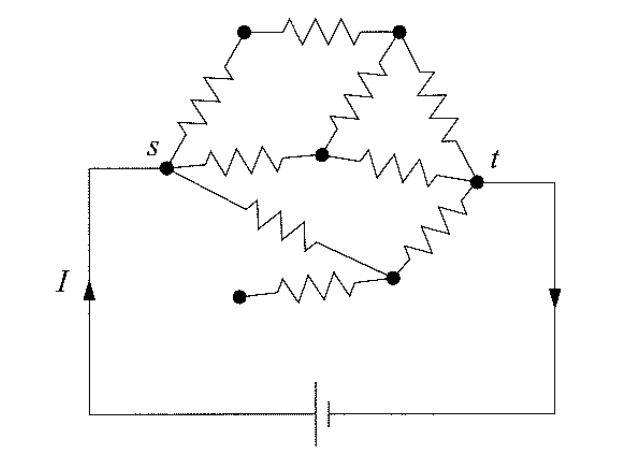
\includegraphics[width=0.5\textwidth]{resistornetwork.png}
   \caption{\label{resistors} Ein Widerstandsnetzwerk. Im Schaltkreis
        flie\ss t der Strom $I$ und alle Widerst\"ande haben den Wert
        $R_0$.} 
        }
\end{figure}


 \subexercise[%
  topic={Allgemeine Netzwerke von Widerst\"anden $R_0$}
    ]

    Schreibe eine Funktion, die als Eingabewerte die Adjazenzmatrix
    $\hat A$, den Einspeiseknoten $s$ und den Ausgangsknoten $t$
    bekommt und als Ausgabe den effektiven Widerstand des Netzwerkes
    berechnet.

    Untersuche die Beziehung des effektiven Widerstandes zwischen
    beliebigen Knoten eines zuf\"alligen Netzwerkes mit Knotenzahl $n$
    und Verbindungswahrscheinlichkeit $p$ zu eben diesen Parametern.



 \exercise[%
     topic={Zusatz) Perkolation von zuf\"alligen Netzwerken},
    ]
    Recherchiere, wie du die Komponenten eines Netzwerkes findest.
    Schreibe eine Funktion, die das f\"ur beliebige Netzwerke tut.

    Generiere zuf\"allige Netzwerke f\"ur variierende Knotenzahlen
    $n$ und Verbindungs\-wahrscheinlichkeiten $p$ und finde den normierten
    Anteil $S$ der gr\"o\ss{}ten Komponente, wobei gilt $S=|V_g|/n$ mit
    der Zahl der Knoten $|V_g|$ in der gr\"o\ss{}ten Komponente
    der Netzwerke (Komponente mit Knoten- und Kantenmenge
    $(V_g,E_g)$).

    Untersuche, wie sich $S$ mit steigendem $p$ f\"ur konstante $n$
    verh\"alt. Wie ist die kritische Wahrscheinlichkeit $p_c$ f\"ur die
    Existenz einer gro\ss{}en Komponente? (Plus Aufgabe von
    vorher: Wie ist der
    mittlere Grad?). 
    
    Erh\"ohe die Knotenzahl. Wie verh\"alt sich $p_c$? Kannst du eine
    Formel f\"ur $p_c$ in Abh\"angigkeit von $n$ und $p$ finden?

    Wie interpretierst du diese?
	
\end{document}
